\documentclass[dvipdfmx,11pt,notheorems]{beamer}
%%%% 和文用 %%%%%
\usepackage{bxdpx-beamer}
\usepackage{pxjahyper}
\usepackage{minijs}%和文用
\renewcommand{\kanjifamilydefault}{\gtdefault}%和文用

%%%% スライドの見た目 %%%%%
\usetheme{Madrid}
\usefonttheme{professionalfonts}
\setbeamertemplate{frametitle}[default][center]
\setbeamertemplate{navigation symbols}{}
\setbeamercovered{transparent}%好みに応じてどうぞ)
\setbeamertemplate{footline}[page number]
\setbeamerfont{footline}{size=\normalsize,series=\bfseries}
\setbeamercolor{footline}{fg=black,bg=black}
%%%%

%%%% 定義環境 %%%%%
\usepackage{amsmath,amssymb}
\usepackage{amsthm}
\theoremstyle{definition}
\newtheorem{theorem}{定理}
\newtheorem{definition}{定義}
\newtheorem{proposition}{命題}
\newtheorem{lemma}{補題}
\newtheorem{corollary}{系}
\newtheorem{conjecture}{予想}
\newtheorem*{remark}{Remark}
\renewcommand{\proofname}{}
\AtBeginSection[]{
    \frame{\tableofcontents[currentsection, hideallsubsections]} %目次スライド
}
% caption に番号追加
\setbeamertemplate{caption}[numbered]
% caption 日本語
\renewcommand{\figurename}{図}
\renewcommand{\tablename}{表}
%%%%%%%%%

%%%%% フォント基本設定 %%%%%
\usepackage[T1]{fontenc}%8bit フォント
\usepackage{textcomp}%欧文フォントの追加
\usepackage[utf8]{inputenc}%文字コードをUTF-8
\usepackage[deluxe,uplatex]{otf}%otfパッケージ
\usepackage[noto,unicode]{pxchfon}
\usepackage{lxfonts}%数式・英文ローマン体を Lxfont にする
\usepackage{bm}%数式太字
\renewcommand{\familydefault}{\sfdefault}
\usefonttheme[onlymath]{serif}
\DeclareSymbolFont{operators}{OT1}{\sfdefault}{m}{n}
\SetSymbolFont{operators}{bold}{OT1}{\sfdefault}{b}{n}
\usefonttheme{structurebold} % タイトル部を太字
\setbeamerfont{alerted text}{series=\bfseries} % Alertを太字
\setbeamerfont{section in toc}{series=\mdseries} % 目次は太字にしない
\setbeamerfont{frametitle}{size=\Large} % フレームタイトル文字サイズ
\setbeamerfont{title}{size=\LARGE} % タイトル文字サイズ
\setbeamerfont{date}{size=\small}  % 日付文字サイズ
%%%%%%%%%%
 
\title[steganograpy]{ステガノグラフィー}%[略タイトル]{タイトル}
\author[ayame]{堀野 智康}%[略名前]{名前}
\institute[KMC]{電気電子工学科3回生}%[略所属]{所属}
\date{2019年1月21日}%日付
\begin{document}

\begin{frame}[plain]\frametitle{}
	\titlepage %表紙
\end{frame}

\begin{frame}\frametitle{内容}
	\tableofcontents %目次
\end{frame}

\section{はじめに}
\begin{frame}\frametitle{デジタル信号処理}
	デジタル信号処理の授業で習ったこと。
	\begin{itemize}
		\item いろいろな直交変換
		      \begin{itemize}
			      \item 離散フーリエ変換
			      \item ウェーブレット変換
			      \item 離散コサイン変換
			      \item ラプラス変換(Z変換)
		      \end{itemize}
		\item 変換した領域で行う操作(おもにフィルタ)
	\end{itemize}

	今からやることも直交変換して周波数領域でちょっとした操作をするだけです。
\end{frame}

\begin{frame}\frametitle{テーマ}
	\begin{block}{やったこと}
		画像に秘密データ(文字列)を隠ぺいするプログラムを作りました。
	\end{block}
	たいそうな言葉遣いだけど、単に画像にばれないように秘密の印
	をつけただけ。
\end{frame}

\begin{frame}\frametitle{経緯}
	JPEGで人間の目に適した圧縮をやっていることから着想
	\begin{itemize}
		\item JPEGでは人間の鈍感な周波数成分をうまく取り除くことで見た目を変えずに圧縮している。
		\item ならば人間の鈍感な周波数成分にデータを隠すことができるのでは?
	\end{itemize}
	ググった結果、どうやらステガノグラフィーというらしい。
\end{frame}

\begin{frame}\frametitle{説明}
	\begin{block}{ステガノグラフィーとは}
		ステガノグラフィー(steganography)とは、データ隠蔽技術の一つであり、データを他のデータに埋め込む技術のこと、あるいはその研究を指す。
		クリプトグラフィー(cryptography)がメッセージの内容を読めなくする手段を提供するのに対して、ステガノグラフィーは存在自体を隠す点が異なる。

		(Wikipediaより)
	\end{block}
	「ニイタカヤマノボレ」がどちらかというとステガノグラフィーで

	"WJRJRGJW UJFWQ MFWGTW"はクリプトグラフィーかな?(よく知らない)
\end{frame}

\section{方法}
\begin{frame}\frametitle{方法}
	\begin{enumerate}
		\item 2次元のカラー画像を読み込む。
		\item 直交変換をする。
		\item 周波数領域で人間の鈍感な高周波成分にデータを埋め込む。
		\item 逆変換して画像に戻す。
	\end{enumerate}
	以上!
\end{frame}

\begin{frame}\frametitle{画像の読み込み}
	\begin{block}{手順1}
		2次元のカラー画像を読み込む。
	\end{block}
	カラー画像はR,G,Bの3色で表され、

	画素もR,G,Bのそれぞれが多くの場合$0\sim 255$(8 bit)の間でデータ(unsigned char)を持つ。
\end{frame}

\begin{frame}\frametitle{直交変換}
	\begin{block}{手順2}
		画像を2次元離散コサイン変換する。
	\end{block}
	カラー画像はR成分のみ,G成分のみ,B成分のみの画像に分けて、

	2次元離散コサイン変換をする。このときスケールを$0\sim 1$で規格化しておく(float)。

	変換式は異なるが方法は2次元離散フーリエ変換と同じ。

	2次元離散コサイン変換は画像全体を$4\times 4$マスのブロックに分割しておこなった。
	このブロックの高周波成分を使用して\,1\,bitのデータを入れていく。
	\begin{exampleblock}{ちょっと一工夫}
		どうやら人間は寒色に鈍感らしいので、
		カラー画像のときは青成分だけをいじるようにしました。
	\end{exampleblock}
\end{frame}

\begin{frame}\frametitle{データの埋め込み}
	\begin{block}{手順3}
		高周波領域にデータを埋め込む。
	\end{block}
	2次元離散コサイン変換をすると高周波成分は右下に出てくるので、

	そこに0,1のデータを高周波成分の新たなDCT係数として与えればよい。自分のプログラムでは
	入れたいデータが 0 のとき 0 、入れたいデータが 1 のとき 0.1 を与えている。

	ここで入れる係数を大きくしすぎると生成画像に粗が出てしまい、
	逆に係数を小さくしすぎると丸め誤差の影響でデータが変化しやすくなる。
\end{frame}

\begin{frame}\frametitle{逆変換}
	\begin{block}{手順4}
		逆変換して画像に戻す。
	\end{block}
	2次元離散コサイン逆変換をする。

	横・縦という順で変換をしたならば縦・横という順で逆変換を施す。
	縦・横という順で変換をしたならば横・縦という順で逆変換を施す。

	画像に戻って出来上がり!
\end{frame}

\section{結果}
\begin{frame}\frametitle{結果(1)}
	右側が情報を埋めた画像。符号誤り率は\,0/49152\,だった。

	\begin{figure}[htbp]
		\begin{center}
			\begin{tabular}{c}

				% 1
				\begin{minipage}{0.5\hsize}
					\begin{center}
						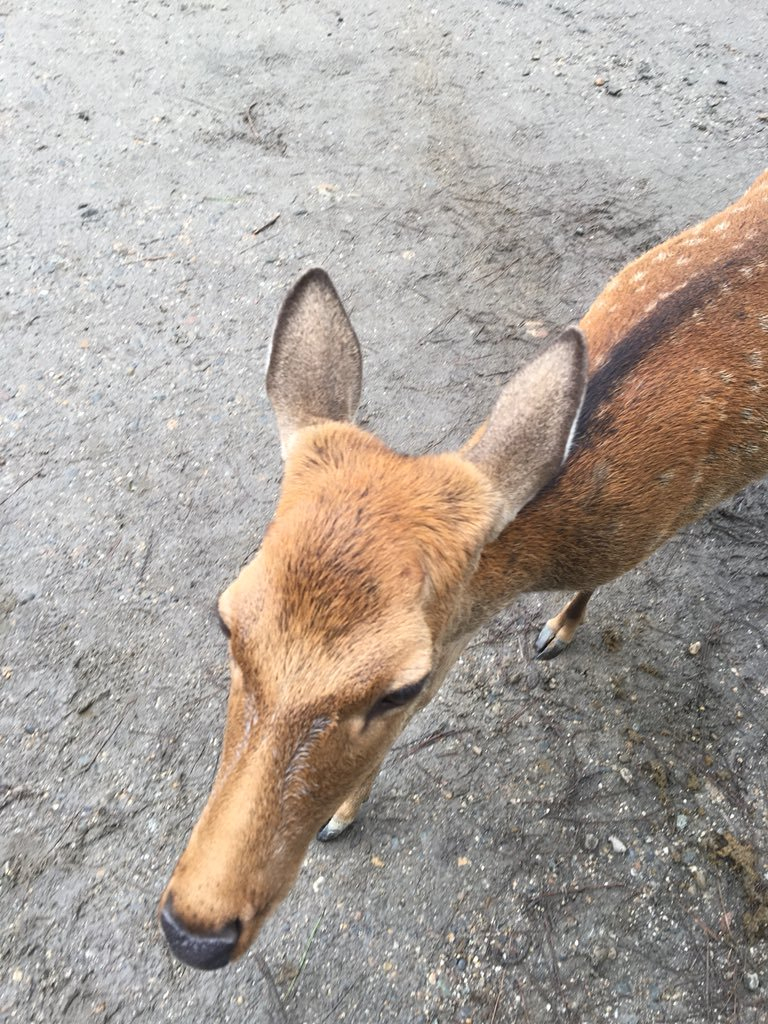
\includegraphics[clip, width=4.5cm]{Nara.jpg}
						\hspace{1.6cm} [1]\ 元データ
					\end{center}
				\end{minipage}

				% 2
				\begin{minipage}{0.5\hsize}
					\begin{center}
						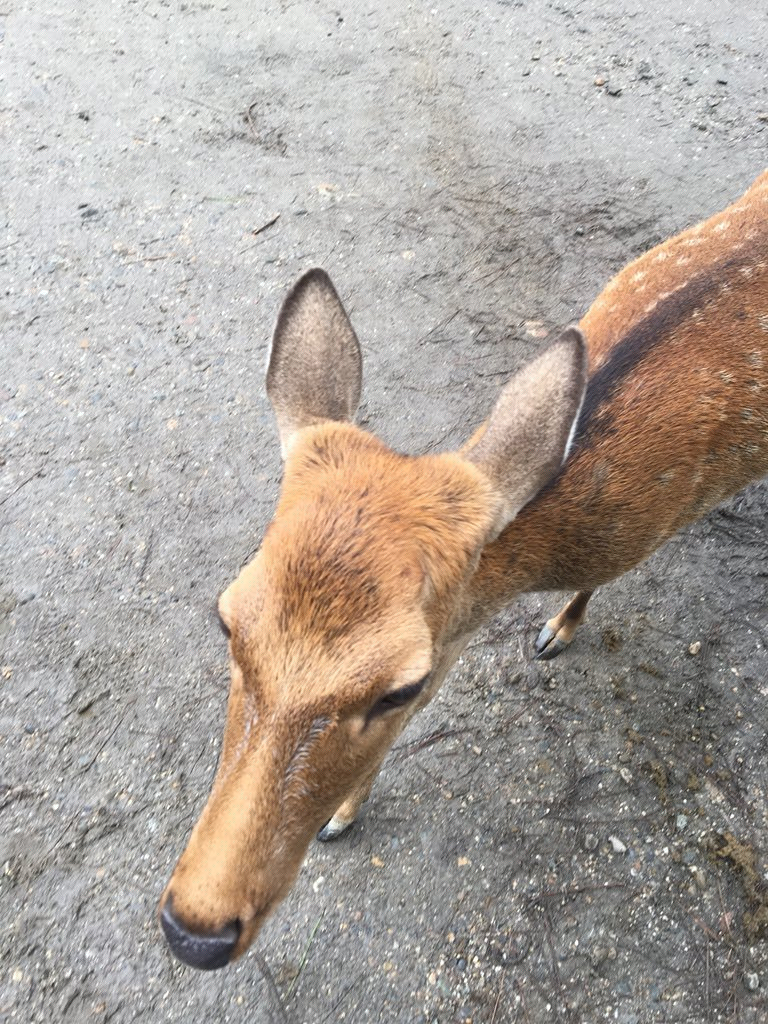
\includegraphics[clip, width=4.5cm]{StegoNara.png}
						\hspace{1.6cm} [2]\ 後データ
					\end{center}
				\end{minipage}
			\end{tabular}
			\caption{奈良公園の鹿}
			\label{fig:nara}
		\end{center}
	\end{figure}
\end{frame}

\begin{frame}{結果(2)}
	ただし、下のような激しい画像では符号誤り率は\,2343/24360\,だった。

	\begin{figure}[htbp]
		\begin{center}
			\begin{tabular}{c}

				% 1
				\begin{minipage}{0.5\hsize}
					\begin{center}
						
\includegraphics[clip, width=4.5cm]{Test.png}
						\hspace{1.6cm} [1]\ 元データ
					\end{center}
				\end{minipage}

				% 2
				\begin{minipage}{0.5\hsize}
					\begin{center}
						
\includegraphics[clip, width=4.5cm]{StegoTest.png}
						\hspace{1.6cm} [2]\ 後データ
					\end{center}
				\end{minipage}
			\end{tabular}
			\caption{よくない画像}
			\label{fig:test}
		\end{center}
	\end{figure}
\end{frame}

\begin{frame}{まとめ}
	\begin{itemize}
		\item 一般的な画像であれば誤りも少なく情報を埋め込むことがえできた。
		\item ぐちゃぐちゃな画像では誤りが大きくなってあまり実用的ではない。
	\end{itemize}
	\begin{alertblock}{注意}
		そもそも明らかに怪しい意味のよくわからない混沌とした画像を\,StegoBox\,
		に選ぶこと自体がよくないので、普通の画像を選びましょう。
	\end{alertblock}
\end{frame}

\section{デモンストレーション}
\begin{frame}\frametitle{デモンストレーション}
	以上スライドによる簡単な説明を終わります。

	残った時間で実際にデータを画像に埋め込んで、取り出してみます。
\end{frame}

\end{document}